\documentclass[12pt]{article}

\usepackage{sbc-template}
\usepackage{graphicx,url}
\usepackage[utf8]{inputenc}
\usepackage[brazil]{babel}
\usepackage{booktabs}
\usepackage{amsmath}

\graphicspath{{figuras/}}

\sloppy

\title{Identificação de Fatores Relevantes para Melhoria de Ranqueamento em SERP a partir de Métricas de SEO}

\author{Felipe Augusto Medici de Oliveira\inst{1}}

\address{Programa de Pós-Graduação em Ciência da Computação (PPGCC)\\
  Universidade Tecnológica Federal do Paraná (UTFPR), Campus Campo Mourão\\
  Campo Mourão, PR, Brasil
  \email{felipemedici@alunos.utfpr.edu.br}
}

\begin{document}

\maketitle

\begin{resumo}
A otimização para mecanismos de busca (SEO) tornou-se estratégica para a visibilidade
de conteúdos digitais, mas nem sempre é evidente quais métricas mais contribuem para a
melhoria de posição nas páginas de resultados (SERP). Este trabalho investiga, por meio
de análise baseada em dados, quais fatores de SEO mais se associam à melhoria de
ranqueamento, formulando o problema como classificação binária supervisionada da variável
\textit{ranking\_improved}. Sobre um conjunto público com 500 instâncias e 13 preditoras,
comparou-se uma bateria de modelos (baseline majoritário, Regressão Logística, k-NN,
SVM-RBF, Random Forest, XGBoost e combinações por \textit{voting} e \textit{stacking})
com pré-processamento livre de vazamento, validação cruzada estratificada repetida, testes
estatísticos de Friedman, Nemenyi e Wilcoxon, e análise de importância de atributos. Os
resultados mostram sinal preditivo fraco: nenhum modelo supera substancialmente o baseline,
e apenas a Regressão Logística obtém ganho estatisticamente significativo em PR-AUC.
Modelos complexos não trouxeram vantagem sob sinal fraco. Por informação mútua, fatores
comportamentais, de autoridade e contextuais lideram a associação com o alvo, enquanto
métricas puramente \textit{on-page} contribuem menos. O estudo evidencia tanto os fatores
mais relevantes quanto os limites da análise preditiva de SEO em dados de baixo sinal.
\end{resumo}

\begin{abstract}
Search engine optimization (SEO) has become strategic for the visibility of digital
content, yet it is often unclear which metrics most contribute to improving a page position
on search engine results pages (SERP). This work investigates, through dataset-based
analysis, which SEO factors are most associated with ranking improvement, framing the task
as supervised binary classification of the \textit{ranking\_improved} target. On a public
dataset with 500 instances and 13 predictors, we compare a battery of models (majority
baseline, Logistic Regression, k-NN, SVM-RBF, Random Forest, XGBoost, and voting and
stacking ensembles) using leakage-free preprocessing, repeated stratified cross-validation,
Friedman, Nemenyi and Wilcoxon statistical tests, and feature importance analysis. Results
reveal a weak predictive signal: no model substantially exceeds the baseline, and only
Logistic Regression achieves a statistically significant PR-AUC gain. Complex models bring
no advantage under weak signal. By mutual information, behavioral, authority and contextual
factors lead the association with the target, while purely on-page metrics contribute less.
The study highlights both the most relevant factors and the limits of predictive SEO
analysis on low-signal data.
\end{abstract}

\section{Introdução}

O crescimento da competição por visibilidade em mecanismos de busca tornou a otimização
para mecanismos de busca, conhecida como SEO (\textit{Search Engine Optimization}), uma
área estratégica para empresas, marcas e produtores de conteúdo digital. Diferentes
métricas relacionadas à estrutura da página, à qualidade do conteúdo, à autoridade do
domínio, aos \textit{backlinks} e ao comportamento dos usuários podem influenciar o
desempenho de uma página nos resultados de busca. No entanto, nem sempre é evidente quais
dessas variáveis possuem maior relevância para a melhoria do ranqueamento na página de
resultados, denominada SERP (\textit{Search Engine Results Page}).

A literatura recente aplica aprendizado de máquina para classificar páginas, estimar
posição e identificar fatores influentes \cite{salminen2019,matosevic2021,saeed2024}. Boa
parte desses trabalhos, contudo, formula o problema como estimativa de posição absoluta ou
grau de otimização, e frequentemente depende da acurácia como métrica principal, sem tratar
desbalanceamento de classes nem realizar análise robusta de importância de atributos. Há,
portanto, uma lacuna na formulação orientada à \textit{melhoria observável} de ranqueamento,
isto é, prever se uma página efetivamente subiu de posição após ajustes de conteúdo, e não
apenas descrever seu estado atual.

Este trabalho aborda essa lacuna investigando padrões em métricas de SEO a partir de um
conjunto de dados estruturado, com foco na variável-alvo \textit{ranking\_improved}, que
indica se uma página melhorou ou não sua posição após ajustes. A tarefa de aprendizado é a
classificação binária supervisionada, em que a classe 1 representa melhoria de ranqueamento
e a classe 0 representa ausência de melhoria. A pergunta de pesquisa que orienta o estudo é:
quais métricas de SEO possuem maior relevância para prever a melhoria do ranqueamento de uma
página em SERP?

As contribuições do trabalho são as seguintes. Primeiro, propõe-se um protocolo experimental
rigoroso e reprodutível, com pré-processamento livre de vazamento, validação cruzada
estratificada repetida e comparação estatística entre modelos. Segundo, avalia-se uma bateria
de classificadores de famílias distintas, incluindo combinações por \textit{voting} e
\textit{stacking}, contra um baseline explícito. Terceiro, analisa-se a importância dos
atributos por permutação e informação mútua, agregando-a por grupos de fatores de SEO.
Quarto, e talvez o resultado mais relevante do ponto de vista crítico, evidencia-se que o
conjunto possui sinal preditivo fraco, o que limita o desempenho de qualquer modelo e revela
um cuidado metodológico necessário em análises de SEO baseadas em dados simulados. Todo o
código e os artefatos estão disponíveis publicamente\footnote{Repositório:
\url{https://github.com/usuario/seo-serp-ranking} (substituir pelo endereço definitivo).}.

O restante do artigo está organizado da seguinte forma. A Seção~\ref{sec:relacionados}
revisa criticamente os trabalhos relacionados e posiciona o estudo frente às lacunas
identificadas. A Seção~\ref{sec:dados} descreve o conjunto de dados. A
Seção~\ref{sec:metodos} detalha materiais e métodos, incluindo o pipeline de
pré-processamento, os algoritmos, a estratégia de combinação de classificadores, o protocolo
de validação e as métricas. A Seção~\ref{sec:resultados} apresenta e discute os resultados,
com comparações entre modelos e análise estatística. A Seção~\ref{sec:conclusao} sintetiza
as contribuições, as limitações e os trabalhos futuros.

\section{Trabalhos Relacionados}
\label{sec:relacionados}

A revisão posiciona o projeto no cruzamento de três frentes: SEO empírico e fatores de
ranqueamento, modelagem preditiva e interpretação para decisão. Em SEO empírico,
\cite{lewandowski2021} mostram que a otimização altera a composição e a visibilidade dos
resultados do Google, enquanto \cite{ali2021} revisam, em perspectiva de conteúdo e estrutura
de links, que os links são relevantes mas insuficientes isoladamente. A evolução das próprias
SERPs, cada vez mais ricas em recursos, é documentada por \cite{duka2023} e
\cite{oliveira2023}, que ressaltam a diversificação de respostas diretas e verticais. Em
qualidade linguística de conteúdo, \cite{cirakoglu2024} discutem dimensões de clareza e
intenção por meio das máximas de Grice, ainda pouco operacionalizáveis sem atributos de
processamento de linguagem natural.

Na modelagem preditiva, \cite{salminen2019} predizem ranqueamento no setor de presentes com
\textit{LightGBM}, \textit{XGBoost} e \textit{learning-to-rank}, apontando o XGBoost como
melhor e destacando links e segurança do domínio via SHAP. \cite{matosevic2021} classificam
páginas por grau de otimização \textit{on-page}, com seleção por ganho de informação e
\textit{Relief}, obtendo acurácias entre 54,6\% e 69,7\% sobre um baseline de 48,8\%.
\cite{attia2022} propõem um modelo multicritério de indexação e ranqueamento em larga escala,
mostrando que combinar critérios supera o critério único. \cite{roumeliotis2023} apresentam
uma ferramenta de auditoria de SEO em Python com aprendizado de máquina, voltada a
recomendações práticas. \cite{saeed2024} exploram fatores de SEO para busca por voz com SVM,
Regressão Logística, \textit{Naive Bayes}, k-NN, árvore de decisão e Random Forest,
destacando o Random Forest e atributos novos sobre baselines. \cite{almadhoun2025} estimam
ranqueamento com árvores, \textit{boosting} e aprendizado profundo, reportando \textit{Gradient
Boosted Trees} com 77,58\% em cenário multiclasse e 86,56\% no binário.

A Tabela~\ref{tab:relacionados} sintetiza esses trabalhos segundo problema, dados, algoritmos,
métricas, principais resultados e a limitação-chave que conecta cada um às lacunas tratadas
neste projeto.

\begin{table}[ht]
\centering
\caption{Síntese comparativa dos trabalhos relacionados.}
\label{tab:relacionados}
\footnotesize
\begin{tabular}{p{2.3cm}p{2.6cm}p{2.4cm}p{2.4cm}p{2.6cm}}
\toprule
\textbf{Referência} & \textbf{Problema} & \textbf{Algoritmos} & \textbf{Métricas} & \textbf{Limitação-chave} \\
\midrule
Salminen (2019) & Predição de ranking (e-commerce) & LightGBM, XGBoost, SHAP & Acurácia ($\approx$0,86), NDCG & Dataset setorial; não mede melhoria temporal \\
Matošević (2021) & Grau de otimização \textit{on-page} & Classificadores supervisionados, RF & Acurácia vs. baseline & Rótulo subjetivo; sem ranking real \\
Lewandowski (2021) & Influência do SEO no Google & Análise observacional & Análise empírica & Sem modelo preditivo \\
Ali \& Khusro (2021) & Revisão de ranking por conteúdo e links & Categorização de algoritmos & Avaliação qualitativa & Sem experimento próprio \\
Attia (2022) & Indexação multicritério & Modelo MCIR & Comparação 1 vs. N & Próximo de IR geral \\
Saeed (2024) & Fatores para busca por voz & SVM, LogReg, NB, k-NN, DT, RF & Acurácia, matriz de confusão & Foco em voz; dependência de \textit{scraping} \\
Almadhoun \& Malim (2025) & Estimação de ranking & DT, k-NN, NB, GBT, XGBoost, RF, DL & Acurácia multiclasse e binária & Estima posição, não melhoria \\
\textbf{Este trabalho} & \textbf{Melhoria de ranking} (\textit{ranking\_improved}) & \textbf{Bateria + ensembles + testes} & \textbf{PR-AUC, F1-macro, ROC-AUC} & \textbf{Trata desbalanceamento e leakage} \\
\bottomrule
\end{tabular}
\end{table}

A análise da cobertura revela lacunas críticas pouco atendidas pelo estado da arte: o foco em
melhoria de ranqueamento, e não em posição ou grau de otimização; o tratamento explícito do
desbalanceamento de classes \cite{he2009}; o uso de métricas robustas em vez de acurácia
isolada \cite{saito2015}; a avaliação de estabilidade da importância de atributos; e o
controle de vazamento de informação. Este projeto posiciona-se exatamente sobre essas lacunas,
reformulando o alvo para a melhoria observável e adotando protocolo de avaliação e
interpretação mais rigoroso do que o usual.

\section{Conjunto de Dados}
\label{sec:dados}

Utiliza-se o \textit{SEO Web Content Dataset}, disponibilizado na plataforma Kaggle, que
simula métricas de SEO de páginas web com foco no impacto de ajustes de conteúdo e de
engajamento sobre o ranqueamento. O conjunto possui 500 instâncias e 14 colunas, sendo 13
preditoras e a variável-alvo \textit{ranking\_improved}. Não há valores ausentes em nenhuma
coluna. As preditoras abrangem fatores de conteúdo (por exemplo, \textit{content\_length} e
\textit{keyword\_density}), de estrutura e \textit{on-page} (\textit{num\_internal\_links},
\textit{has\_meta\_description}, \textit{has\_alt\_text}), de autoridade e \textit{off-page}
(\textit{domain\_authority}, \textit{page\_authority}, \textit{backlink\_count},
\textit{num\_external\_links}), comportamentais (\textit{avg\_time\_on\_page\_sec},
\textit{bounce\_rate}, \textit{scroll\_depth\_percent}) e contextuais
(\textit{serp\_position\_before}).

A variável-alvo apresenta leve desbalanceamento, com 312 instâncias na classe 0 (62,4\%) e
188 na classe 1 (37,6\%), como ilustra a Figura~\ref{fig:dist}. Esse fator exige cautela na
avaliação, evitando o uso isolado da acurácia. A análise preliminar mostrou correlações
lineares fracas entre as preditoras e o alvo, com coeficiente de Pearson de magnitude máxima
em torno de 0,09 (Figura~\ref{fig:corr}). Tal característica sugere que eventuais relações
úteis não são puramente lineares, o que motiva o uso de modelos capazes de capturar padrões
mais complexos e de medidas de associação não lineares, como a informação mútua.

\begin{figure}[ht]
\centering
\begin{minipage}{0.46\textwidth}
\centering
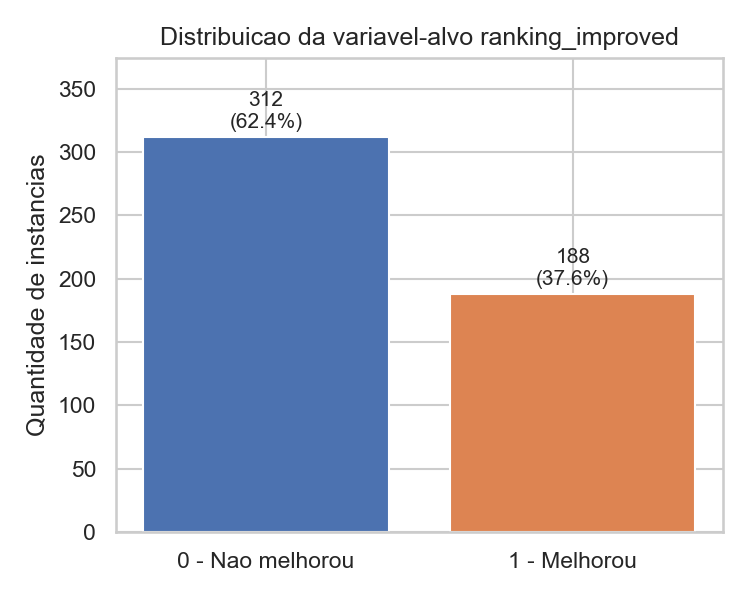
\includegraphics[width=\textwidth]{class_distribution.png}
\caption{Distribuição da variável-alvo.}
\label{fig:dist}
\end{minipage}\hfill
\begin{minipage}{0.50\textwidth}
\centering
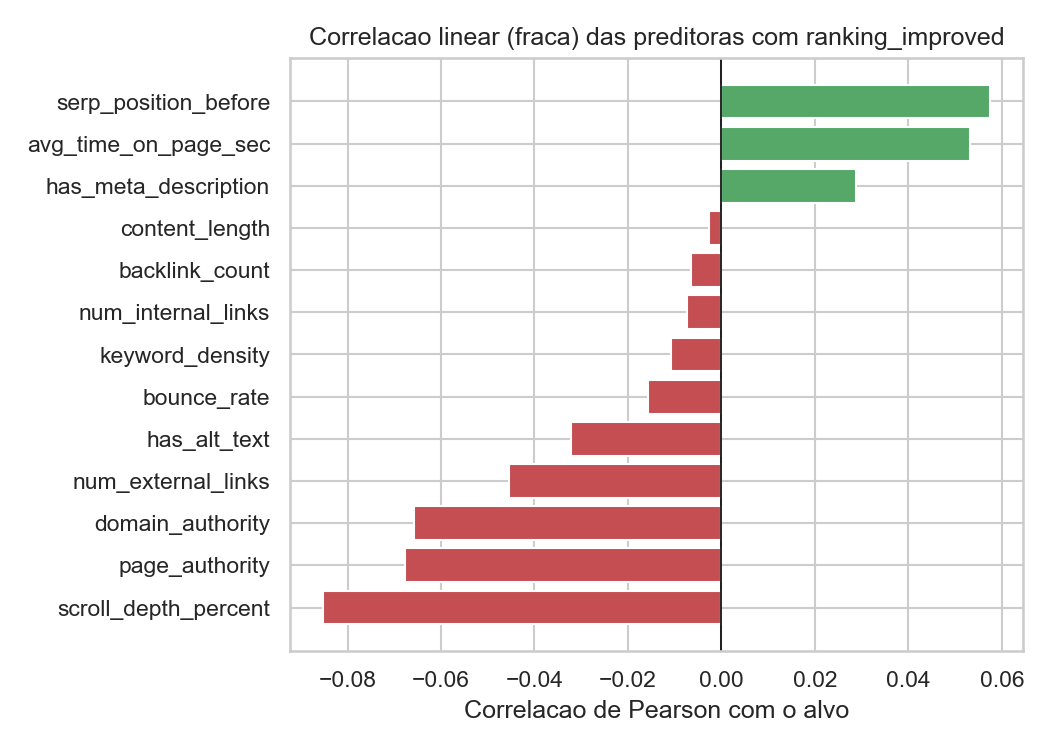
\includegraphics[width=\textwidth]{target_correlation.png}
\caption{Correlação linear (fraca) com o alvo.}
\label{fig:corr}
\end{minipage}
\end{figure}

Quatro características do dado guiam as decisões metodológicas. A correlação linear fraca
recomenda priorizar modelos não lineares e usar informação mútua. O desbalanceamento leve
indica que a acurácia isolada engana, devendo ser tratado preferencialmente por ponderação de
classes antes de reamostragem agressiva. O volume reduzido, de apenas 500 linhas, desaconselha
\textit{undersampling} e favorece validação cruzada em vez de uma única partição de teste. Por
fim, como o objetivo é descobrir fatores, mantêm-se atributos interpretáveis, sem aplicar
projeções como PCA ou LDA no pipeline de modelagem. A licença de uso deve ser confirmada na
página do Kaggle antes de qualquer redistribuição.

\section{Materiais e Métodos}
\label{sec:metodos}

\subsection{Pipeline de pré-processamento}

O princípio que orienta todo o pipeline é a prevenção de vazamento de informação: o
escalonamento, a seleção e a reamostragem são ajustados somente no fold de treino, dentro da
validação cruzada, encapsulados em objetos \textit{Pipeline} do \textit{scikit-learn} e do
\textit{imbalanced-learn} \cite{pedregosa2011}. Nada é ajustado sobre o conjunto completo antes
da partição. A ausência de valores faltantes foi confirmada programaticamente. Como as escalas
das preditoras diferem bastante, aplica-se padronização por escore z aos modelos lineares, de
distância e de margem, ao passo que as árvores, invariantes à escala, não recebem
escalonamento. Não há necessidade de codificação de variáveis, pois as 13 preditoras são
numéricas ou já binárias em $\{0,1\}$. A extração de atributos por componentes foi descartada
por destruir a interpretabilidade, que é central ao objetivo do trabalho.

O desbalanceamento leve foi tratado de forma escalonada e comparada. A primeira opção, sem
geração de dados sintéticos, é a ponderação de classes por \texttt{class\_weight='balanced'};
em seguida, avalia-se a sobreamostragem sintética SMOTE \cite{chawla2002}. O
\textit{undersampling} puro foi descartado, pois descartar dados é custoso em uma amostra
pequena. De forma crítica, a reamostragem é aplicada apenas ao fold de treino, por meio de um
\textit{Pipeline} do \textit{imbalanced-learn}, o que evita o vazamento típico da reamostragem
feita sobre o conjunto inteiro. O atributo \textit{serp\_position\_before} é um preditor
legítimo, mas pode atuar como confundidor com efeito de teto, já que uma página no topo tem
pouca margem para melhorar. Por isso, conduz-se uma análise de ablação com e sem esse atributo.

\subsection{Algoritmos e combinação de classificadores}

Adota-se a progressão baseline, linear, árvore e \textit{ensemble}, cobrindo famílias distintas
para testar a hipótese de que combinações superam modelos lineares. O baseline é um
\textit{DummyClassifier} que prevê sempre a classe majoritária, definindo o piso de 62,4\% de
acurácia. A Regressão Logística fornece coeficientes interpretáveis e serve de referência
linear. O Random Forest \cite{breiman2001} captura não linearidades e interações sem
padronização, com importância nativa de atributos. O XGBoost \cite{chen2016} representa o
estado da arte em dados tabulares e integra-se naturalmente a análises de importância. Como
modelos complementares exploratórios, avaliam-se SVM com \textit{kernel} RBF e k-NN. O
desbalanceamento é tratado por ponderação de classes nos modelos do \textit{scikit-learn} e por
\texttt{scale\_pos\_weight} aproximadamente igual a 1,66 no XGBoost.

A combinação de classificadores é avaliada por \textit{Soft Voting} sobre Regressão Logística,
Random Forest e XGBoost, e por \textit{Stacking} com base em Random Forest, XGBoost e SVM e
meta-aprendiz de Regressão Logística, cuja meta-camada é treinada por validação cruzada interna
para evitar vazamento. Os hiperparâmetros dos modelos principais são ajustados por busca
aleatória (\textit{RandomizedSearchCV}) na validação cruzada interna, explorando, por exemplo,
o termo de regularização da Regressão Logística, a profundidade e o número de árvores do Random
Forest, e a taxa de aprendizado, a profundidade e a subamostragem do XGBoost.

\subsection{Protocolo de validação e métricas}

Com 500 instâncias, uma única partição de teste seria instável. Adota-se validação cruzada
estratificada aninhada, com laço externo de 5 folds para estimativa não enviesada e laço interno
de 3 folds para o ajuste de hiperparâmetros. A estratificação preserva a proporção 62/38 em cada
fold. Para a comparação principal entre modelos, utiliza-se validação cruzada estratificada
repetida, com 5 folds e 3 repetições, totalizando 15 medidas por modelo e conferindo maior poder
aos testes estatísticos. Um holdout estratificado de 20\% é reservado apenas como confirmação
final, do qual se reporta uma matriz de confusão.

A acurácia isolada é descartada como métrica principal devido ao desbalanceamento. Reporta-se,
como métrica primária, a PR-AUC, que foca a classe minoritária de interesse
\cite{saito2015}; e, de forma complementar, F1-macro, Balanced Accuracy, ROC-AUC, além de
precisão, revocação e F1 da classe positiva. O modelo campeão é definido pela maior PR-AUC média
na validação cruzada externa, com desempate por F1-macro. Para afirmar superioridade não
casual, aplica-se o teste de Friedman seguido do pós-teste de Nemenyi com diagrama de diferença
crítica \cite{demsar2006}, além do teste de Wilcoxon pareado de cada modelo contra o baseline,
ao nível de significância de 0,05. A interpretabilidade é tratada por importância de permutação
agregada em folds, cujo desvio mede a estabilidade do ranking de atributos, complementada por
informação mútua e por agregação por grupo de fatores. A reprodutibilidade é garantida por
sementes fixas, versões de bibliotecas registradas e todo o pré-processamento encapsulado em
\textit{Pipeline}.

\section{Resultados e Discussão}
\label{sec:resultados}

\subsection{Comparação entre modelos}

A Tabela~\ref{tab:modelos} apresenta o desempenho médio dos modelos na validação cruzada
estratificada repetida. O resultado central é que o sinal preditivo do conjunto é fraco:
nenhum modelo supera substancialmente o baseline, e os valores de ROC-AUC permanecem próximos
de 0,5, indicando capacidade discriminativa reduzida. A Regressão Logística obtém a maior
PR-AUC média (0,413) e o melhor rank médio, seguida de k-NN, Random Forest e SVM-RBF. A
Figura~\ref{fig:box} mostra a distribuição da PR-AUC por fold.

\begin{table}[ht]
\centering
\caption{Desempenho médio na validação cruzada estratificada repetida (5 $\times$ 3). Valores em negrito indicam o melhor por coluna.}
\label{tab:modelos}
\small
\begin{tabular}{lcccccc}
\toprule
\textbf{Modelo} & \textbf{PR-AUC} & \textbf{ROC-AUC} & \textbf{F1-macro} & \textbf{Bal. Acc.} & \textbf{Recall (1)} & \textbf{Acurácia} \\
\midrule
Dummy (majoritária) & 0,376 & 0,500 & 0,384 & 0,500 & 0,000 & 0,624 \\
Regressão Logística & \textbf{0,413} & 0,504 & \textbf{0,500} & \textbf{0,505} & \textbf{0,470} & 0,514 \\
k-NN & 0,396 & 0,499 & 0,470 & 0,503 & 0,156 & 0,589 \\
SVM-RBF & 0,396 & 0,471 & 0,474 & 0,478 & 0,399 & 0,497 \\
Random Forest & 0,391 & \textbf{0,504} & 0,444 & 0,499 & 0,098 & 0,598 \\
XGBoost & 0,383 & 0,481 & 0,476 & 0,479 & 0,296 & 0,525 \\
Soft Voting & 0,391 & 0,492 & 0,477 & 0,485 & 0,252 & 0,543 \\
Stacking & 0,372 & 0,463 & 0,384 & 0,500 & 0,000 & 0,623 \\
\bottomrule
\end{tabular}
\end{table}

\begin{figure}[ht]
\centering
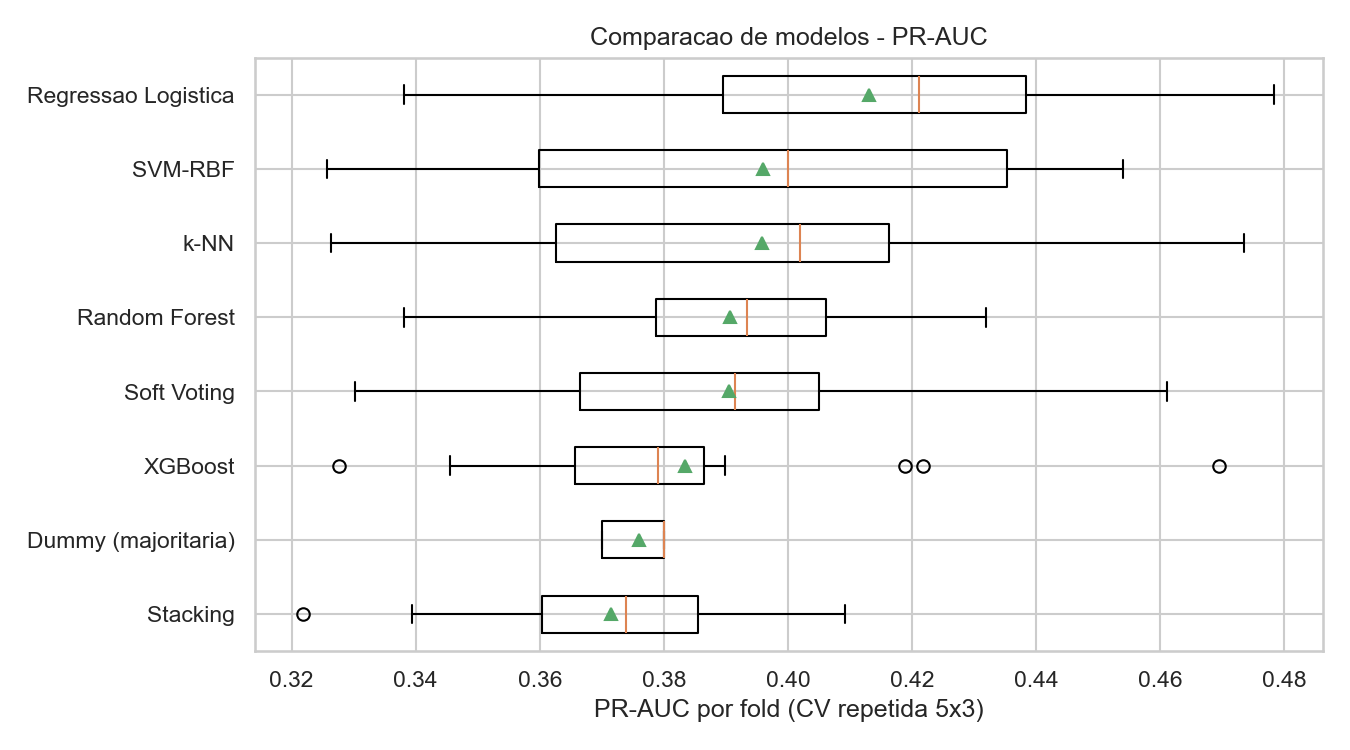
\includegraphics[width=0.78\textwidth]{model_comparison_prauc.png}
\caption{Distribuição da PR-AUC por fold para cada modelo na validação cruzada repetida.}
\label{fig:box}
\end{figure}

Um achado relevante é que os modelos complexos não trouxeram vantagem. O Random Forest, o
XGBoost e o \textit{Stacking} ficaram no nível do baseline ou abaixo dele em PR-AUC, e o
\textit{Stacking}, em particular, colapsou na predição da classe majoritária, com revocação
nula para a classe positiva. Esse comportamento é coerente com a teoria: sob sinal fraco e
amostra pequena, modelos de alta capacidade tendem a ajustar ruído, sem ganho de generalização.
A hipótese inicial de superioridade de \textit{ensembles} sobre modelos lineares, portanto, não
se confirma neste conjunto.

\subsection{Análise estatística}

O teste de Friedman indica diferença global significativa entre os modelos
($\chi^2 = 19{,}0$, $p = 0{,}008$). A Tabela~\ref{tab:wilcoxon} apresenta o teste de Wilcoxon
de cada modelo contra o baseline, em PR-AUC pareada por fold. Apenas a Regressão Logística
supera o baseline de forma estatisticamente significativa ($p = 0{,}003$, ganho médio de
0,037 em PR-AUC). Os demais modelos não apresentam diferença significativa, o que reforça a
leitura de sinal fraco. A Figura~\ref{fig:cd} apresenta o diagrama de diferença crítica do
pós-teste de Nemenyi, no qual a Regressão Logística ocupa o melhor rank médio.

\begin{table}[ht]
\centering
\caption{Teste de Wilcoxon de cada modelo contra o baseline (PR-AUC pareada por fold).}
\label{tab:wilcoxon}
\small
\begin{tabular}{lccc}
\toprule
\textbf{Modelo} & \textbf{PR-AUC média} & \textbf{$\Delta$ vs. baseline} & \textbf{Wilcoxon $p$} \\
\midrule
Regressão Logística & 0,413 & $+0{,}037$ & \textbf{0,003} \\
SVM-RBF & 0,396 & $+0{,}020$ & 0,064 \\
Random Forest & 0,391 & $+0{,}015$ & 0,055 \\
k-NN & 0,396 & $+0{,}020$ & 0,188 \\
Soft Voting & 0,391 & $+0{,}015$ & 0,121 \\
XGBoost & 0,383 & $+0{,}007$ & 0,639 \\
Stacking & 0,372 & $-0{,}004$ & 0,600 \\
\bottomrule
\end{tabular}
\end{table}

\begin{figure}[ht]
\centering
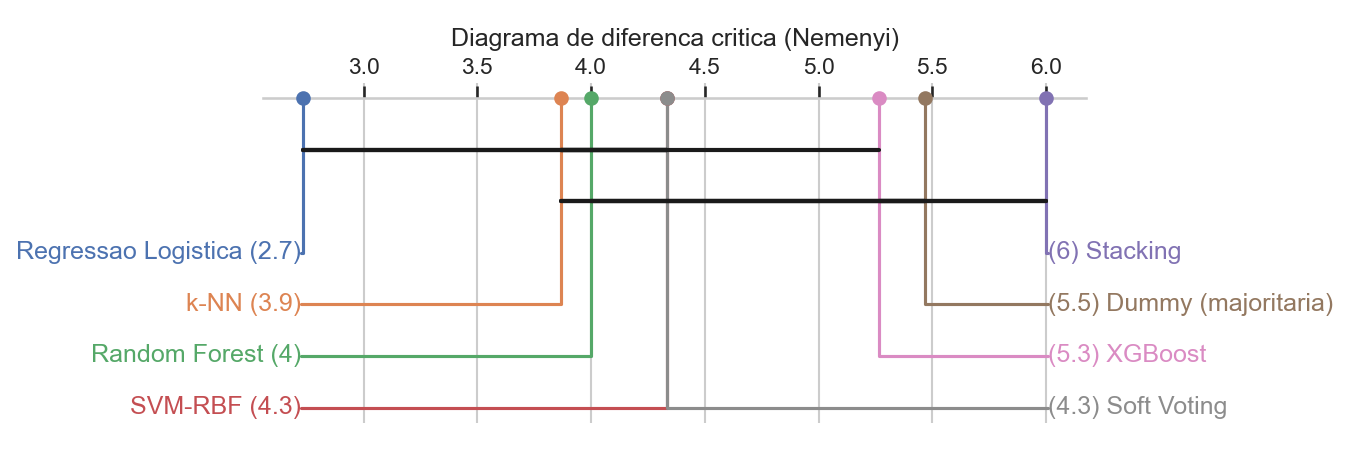
\includegraphics[width=0.85\textwidth]{critical_difference.png}
\caption{Diagrama de diferença crítica (pós-teste de Nemenyi) sobre os ranks médios de PR-AUC.}
\label{fig:cd}
\end{figure}

\subsection{Balanceamento e ajuste de hiperparâmetros}

A Tabela~\ref{tab:balanceamento} compara a ponderação de classes e o SMOTE. Para a Regressão
Logística, a ponderação de classes supera o SMOTE em PR-AUC e em revocação da classe positiva.
Para o Random Forest, o SMOTE aumenta a revocação da classe positiva, de 0,098 para 0,293, ao
custo de redução na PR-AUC. Em síntese, a reamostragem sintética não melhora a métrica primária
neste conjunto, confirmando que, sob desbalanceamento leve, a ponderação de classes é uma
escolha mais segura. A validação cruzada aninhada com hiperparâmetros ajustados manteve os
modelos próximos do baseline, com PR-AUC de 0,391 para a Regressão Logística, 0,386 para o
Random Forest e 0,370 para o XGBoost, o que indica que o ajuste fino não foi capaz de extrair
sinal adicional relevante.

\begin{table}[ht]
\centering
\caption{Comparação de estratégias de balanceamento (validação cruzada repetida).}
\label{tab:balanceamento}
\small
\begin{tabular}{lcccc}
\toprule
\textbf{Estratégia} & \textbf{PR-AUC} & \textbf{Recall (1)} & \textbf{F1 (1)} & \textbf{F1-macro} \\
\midrule
LogReg + ponderação de classes & \textbf{0,413} & 0,470 & \textbf{0,420} & \textbf{0,500} \\
LogReg + SMOTE & 0,398 & 0,457 & 0,412 & 0,496 \\
RF + ponderação de classes & 0,391 & 0,098 & 0,151 & 0,444 \\
RF + SMOTE & 0,368 & 0,293 & 0,315 & 0,475 \\
\bottomrule
\end{tabular}
\end{table}

\subsection{Confirmação em holdout}

No holdout estratificado de 20\%, a Regressão Logística, modelo campeão, alcançou acurácia de
0,510, Balanced Accuracy de 0,513, revocação de 0,526 e F1 de 0,449 para a classe positiva. A
matriz de confusão (Figura~\ref{fig:cm}) e as curvas ROC e Precision-Recall
(Figura~\ref{fig:curvas}) confirmam o padrão observado na validação cruzada: o modelo identifica
parte das melhorias reais, mas a custo de muitos falsos positivos, com desempenho global próximo
ao aleatório. Esse resultado de holdout é consistente com a estimativa por validação cruzada, o
que reforça a validade interna do protocolo.

\begin{figure}[ht]
\centering
\begin{minipage}{0.40\textwidth}
\centering
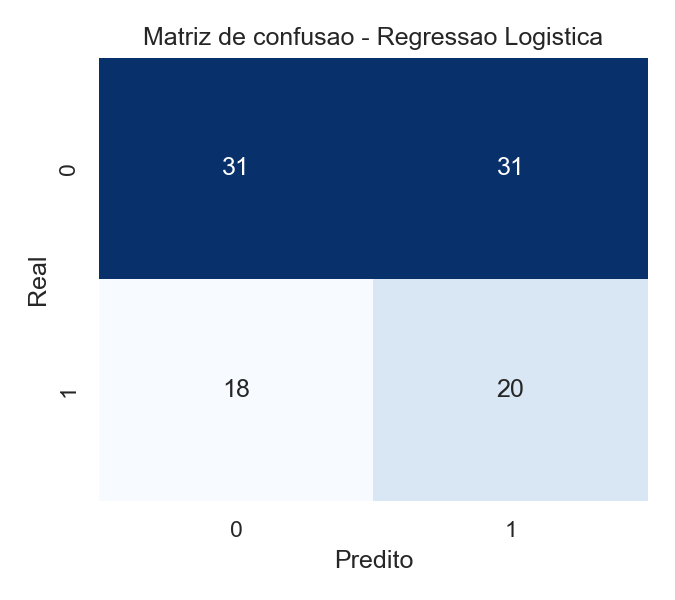
\includegraphics[width=\textwidth]{confusion_matrix.png}
\caption{Matriz de confusão no holdout.}
\label{fig:cm}
\end{minipage}\hfill
\begin{minipage}{0.56\textwidth}
\centering
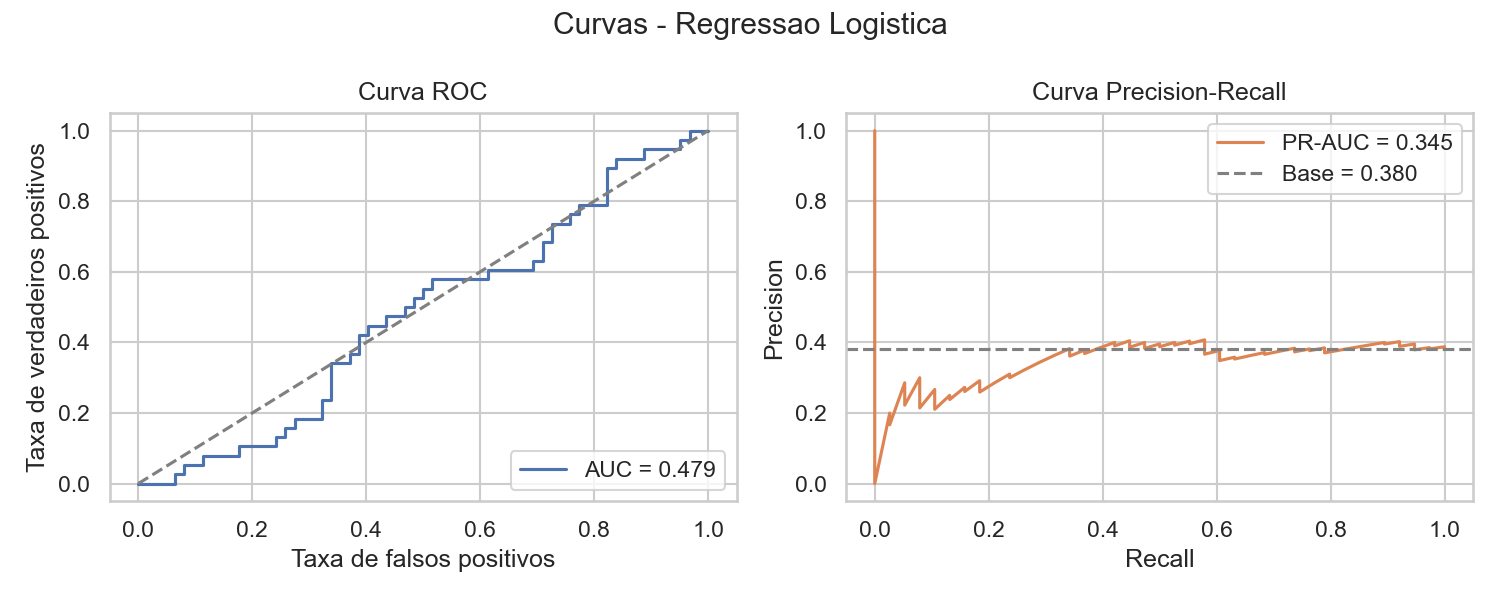
\includegraphics[width=\textwidth]{roc_pr_curves.png}
\caption{Curvas ROC e Precision-Recall no holdout.}
\label{fig:curvas}
\end{minipage}
\end{figure}

\subsection{Importância dos fatores}

A pergunta de pesquisa motiva a análise de importância. A importância por permutação, agregada
em folds, resultou em valores pequenos e instáveis, com desvios da mesma ordem de grandeza das
médias, o que é coerente com o sinal fraco e indica que nenhum atributo isolado domina a
predição. Por essa razão, recorre-se também à informação mútua, calculada sobre todo o conjunto
e mais estável, cuja agregação por grupo é apresentada na Tabela~\ref{tab:grupos} e na
Figura~\ref{fig:grupo}. Os fatores comportamentais, em especial o tempo médio na página e a taxa
de rejeição, e os de autoridade, como a autoridade do domínio e a contagem de \textit{backlinks},
lideram a associação com o alvo, seguidos do fator contextual de posição anterior na SERP. As
métricas puramente \textit{on-page}, como densidade de palavra-chave e presença de meta
description, apresentam associação muito baixa. Esse padrão sustenta a leitura de que sinais de
autoridade e de engajamento se associam mais à melhoria do que ajustes superficiais de conteúdo,
em linha com parte da literatura \cite{salminen2019,saeed2024}.

\begin{table}[ht]
\centering
\caption{Importância agregada por grupo de fatores (informação mútua).}
\label{tab:grupos}
\small
\begin{tabular}{lc}
\toprule
\textbf{Grupo de fatores} & \textbf{Importância total (MI)} \\
\midrule
Comportamental (tempo, rejeição, rolagem) & 0,068 \\
Autoridade (domínio, página, backlinks, links externos) & 0,065 \\
Contextual (posição anterior na SERP) & 0,035 \\
On-page (conteúdo, palavra-chave, meta, links internos) & 0,025 \\
\bottomrule
\end{tabular}
\end{table}

\begin{figure}[ht]
\centering
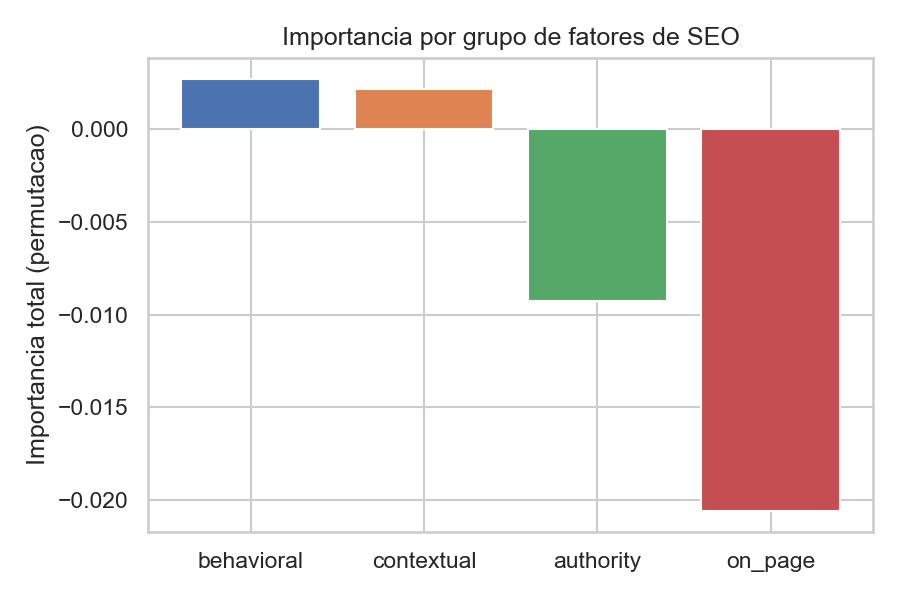
\includegraphics[width=0.62\textwidth]{group_importance.png}
\caption{Importância por grupo de fatores de SEO segundo a importância por permutação do modelo campeão.}
\label{fig:grupo}
\end{figure}

A análise de ablação do atributo \textit{serp\_position\_before} mostrou impacto pequeno: a
PR-AUC variou de 0,413, com o atributo, para 0,409, sem ele. Esse resultado indica que o
atributo é um preditor fraco e legítimo, sem caracterizar um vazamento dominante por efeito de
teto, o que afasta a principal ameaça de confundimento prevista para o conjunto.

\subsection{Discussão e ameaças à validade}

Os resultados respondem à pergunta de pesquisa em dois níveis. No nível dos fatores, os grupos
comportamental, de autoridade e contextual concentram a associação com a melhoria de
ranqueamento, enquanto fatores \textit{on-page} contribuem pouco. No nível metodológico, o
estudo evidencia que o conjunto possui baixo poder preditivo, de modo que modelos sofisticados
não superam um baseline simples nem um modelo linear regularizado. Esse é um resultado honesto e
informativo, que alerta para o risco de superestimar a previsibilidade de SEO em dados
simulados.

Três ameaças à validade merecem registro. A primeira é a natureza simulada do conjunto, cujos
padrões podem não refletir SERPs reais e cuja correlação fraca indica sinal baixo; a mitigação
adotada foi comparar sempre com o baseline e reportar ganhos pequenos de forma transparente. A
segunda é o tamanho reduzido da amostra, com 500 instâncias, que limita modelos de alta
capacidade e o poder estatístico; a mitigação foi a validação cruzada repetida e o uso
exploratório de modelos complexos. A terceira é o possível confundimento de
\textit{serp\_position\_before}, tratado pela ablação. Por fim, o conjunto não possui colunas de
domínio, palavra-chave ou tempo, de modo que protocolos como \textit{GroupKFold} por domínio ou
divisão temporal não se aplicam, e a hipótese de variação da importância por categoria de página
não pôde ser testada.

\section{Conclusão}
\label{sec:conclusao}

Este trabalho investigou, por análise baseada em dados, quais fatores de SEO mais se associam à
melhoria de ranqueamento em SERP, formulando o problema como classificação binária da variável
\textit{ranking\_improved}. As contribuições incluem um protocolo experimental reprodutível e
livre de vazamento, a comparação estatisticamente fundamentada de uma bateria de modelos, e a
análise de importância de atributos por permutação e informação mútua, agregada por grupos de
fatores. Os resultados mostraram que o conjunto possui sinal preditivo fraco, que apenas a
Regressão Logística supera o baseline de forma significativa e que modelos complexos não trazem
vantagem sob essas condições. Quanto aos fatores, sinais comportamentais, de autoridade e
contextuais lideram a associação com o alvo, ao passo que métricas puramente \textit{on-page}
contribuem pouco.

As limitações relacionam-se principalmente à natureza simulada e ao tamanho do conjunto, além da
ausência de atributos que permitiriam protocolos de validação por grupo e análises por categoria.
Como trabalhos futuros, pretende-se validar o protocolo em dados reais de SERP, coletados ao longo
do tempo, incorporar atributos de processamento de linguagem natural e de experiência de página,
e estender a análise de interpretabilidade com SHAP e estudos de estabilidade entre coortes. A
tradução dos fatores mais relevantes em recomendações práticas e priorizadas de SEO permanece um
objetivo central para conectar a modelagem à tomada de decisão orientada por evidências.

\section*{Disponibilidade e uso de IA generativa}

O código-fonte, os dados e os artefatos de resultados estão disponíveis publicamente no
repositório \url{https://github.com/femedici/seo-serp-ranking}. O desenvolvimento empregou
ativamente a abordagem de \textit{Spec Driven Development}, na qual cada etapa partiu de
especificações escritas que orientaram o trabalho com modelos de linguagem. As atividades foram
conduzidas com o \textit{Claude Code}, interface agêntica de linha de comando da Anthropic,
utilizando o modelo \textit{Claude Opus 4.8}. A partir das especificações, os modelos de
linguagem foram empregados para montar agentes de busca sobre o tema, estruturar o projeto,
definir e avaliar métodos e algoritmos de reconhecimento de padrões, gerar e testar o
código-fonte com diferentes metodologias experimentais, e revisar a redação e a organização do
trabalho. O uso concentrou-se em dois eixos principais: a criação e a verificação do código dos
experimentos e a otimização do estudo, o que inclui a comparação entre modelos, o protocolo de
avaliação e a estruturação do texto científico. Todo o conteúdo técnico, os experimentos e os
resultados relatados foram revisados e verificados pelo autor.

\bibliographystyle{sbc}
\bibliography{referencias}

\end{document}
